\documentclass{article}
%packages
% \usepackage{tocloft}
\usepackage{polski}
\usepackage{amsmath}
\usepackage[utf8]{inputenc}
\usepackage{graphicx}
\usepackage{indentfirst}
\usepackage{float}
\usepackage[font=small,labelfont=bf]{caption}
\usepackage[polish]{babel}
\usepackage{hyperref}
\hypersetup{
    colorlinks,
    citecolor=black,
    filecolor=black,
    linkcolor=black,
    urlcolor=black
}
% Variables
\newcommand{\HRule}{\rule{\linewidth}{0.5mm}}
\newcommand{\Prowadzacy}{dr inż. Krzysztof \textsc{Rojek}}
\newcommand{\Ja}{Piotr \textsc{Filek}\\101311\\I grupa}
\newcommand{\DataLaboratorium}{11 października 2013}
\newcommand{\Uczelnia}{ \textsc{\LARGE Politechnika Częstochowska}\\[1.5cm]}
\newcommand{\Przedmiot}{ \textsc{\Large Grafika Komputerowa i Wizualizacja}\\[1.5cm]}
\newcommand{\TytulLaboratirum}{Laboratorium 1\&2\\GIMP}
\frenchspacing

\setlength{\intextsep}{20pt plus 1.0pt minus 2.0pt}

%Equations list
% \newcommand{\listequationsname}{List of Equations}
% \newlistof{myequations}{equ}{\listequationsname}
% \newcommand{\myequations}[1]{%
% \addcontentsline{equ}{myequations}{\protect\numberline{\theequation}#1}\par}

\begin{document}
\begin{titlepage}
\begin{center}
\Uczelnia
% \textsc{\LARGE Politechnika Częstochowska}\\[1.5cm]
\Przedmiot% \textsc{\Large Final year project}\\[0.5cm]
\HRule\\[0.4cm]
{ \huge \bfseries \TytulLaboratirum \\[0.4cm] }
% { \huge \bfseries Large brewing techniques \\[0.4cm]}
\HRule\\[1.5cm]

% Author and supervisor
\begin{minipage}[t]{0.4\textwidth}
\begin{flushleft}\large
\emph{Autor:}\\
\Ja
\end{flushleft}
\end{minipage}
\begin{minipage}[t]{0.5\textwidth}
\begin{flushright} \large
\emph{Prowadzący:} \\
\Prowadzacy
\end{flushright}
\end{minipage}

\vfill

% Bottom of the page
{\large \DataLaboratorium}

\end{center}
\end{titlepage}
% \begin{tableofcontents}
%   \listoffigures
% \end{tableofcontents}
\newpage
\section{Cel laboratorium}
Celem laboratorium było zapoznanie się z obsługą działania programu \emph{GIMP} (ang. \textit{GNU Image Manipulation Program}), programem do tworzenia i edycji grafiki bitmapowej.
\section{Przebieg laboratorium}

Podczas laboratorium zapoznaliśmy się z:
\begin{enumerate}[)]
\item Działaniem na warstwach
\item 
\end{enumerate}

% \begin{figure}[H]
%   \centering
%   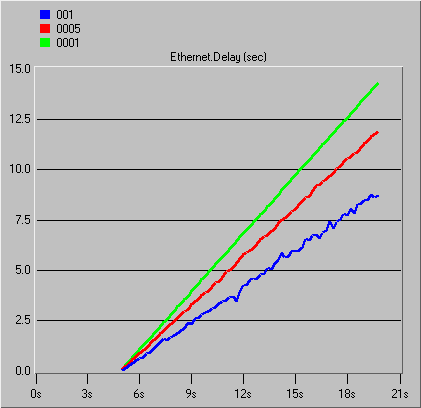
\includegraphics[width=0.65\textwidth]{screens/samo/delay.png}
%   \caption{Wykres przedstawiający opóźnienia.}
%   \label{fig:delay}
% \end{figure}

\section{Wnioski}

\end{document}